\documentclass[UTF8,a4paper,11pt]{ctexart}
\usepackage[left=2.50cm, right=2.50cm, top=2.50cm, bottom=2.50cm]{geometry} %页边距
\CTEXsetup[format={\Large\bfseries}]{section} 
 

% compile using Xelatex
%%%%%%%%%%%%%%%%%%%%%%%   字体备选栏
% -- 中文字体 --
%\setmainfont{Microsoft YaHei}  % 微软雅黑
%\setmainfont{YouYuan}  % 幼圆    
%\setmainfont{NSimSun}  % 新宋体
%\setmainfont{KaiTi}    % 楷体
%\setmainfont{SimSun}   % 宋体
%\setmainfont{SimHei}   % 黑体
% -- 英文字体 --
%\usepackage{times}
%\usepackage{mathpazo}
%\usepackage{fourier}
%\usepackage{charter}
\usepackage{helvet}
 
\usepackage{amsmath, amsfonts, amssymb} % math equations, symbols
\usepackage[english]{babel}
\usepackage{color}      % 控制文本颜色
\usepackage{graphicx}   % 加载图像包
\usepackage{url}        % 网址超链接
\usepackage{bm}         % equations的粗体形式
\usepackage{tikz}       % tikz 图像包
\usepackage{multirow}	% 列表设置一格多行多列
\usepackage{ulem}
\usepackage{booktabs}
\usepackage{epstopdf}
\usepackage{epsfig}
\usepackage{algorithm}  %编写算法

\usepackage{hyperref} %此处设置文本内超链接

%\usepackage{CJK,pgf,pgfarrows,pgfnodes,pgfautomata,pgfheaps}
\usepackage{amsmath,amssymb}
\usepackage{geometry}%页面设置
\usepackage{graphicx}%图片设置
\usepackage{float} %指定图片位置
%\usepackage{subfig}%多个子图
\usepackage{subfigure}%并排子图 共享标题 有子标题
\usepackage{caption}%注释设置

\usepackage{algorithm}
\usepackage{algorithmicx}
\usepackage{algpseudocode}  

% 这个和algorithmic不兼容,用了就要报错,好多莫名其妙的错误!!!!!
\floatname{algorithm}{算法}  
\renewcommand{\algorithmicrequire}{\textbf{输入:}}  
\renewcommand{\algorithmicensure}{\textbf{输出:}}  
\renewcommand{\algorithmicrequire}{ \textbf{Input:}}     %Use Input in the format of Algorithm
\renewcommand{\algorithmicensure}{ \textbf{Output:}}    %UseOutput in the format of Algorithm

\newtheorem{pf}{Pf}
\newtheorem{sol}{Sol}[section]
\newtheorem{thm}{Thm}
\newtheorem{ex}{e.g.}
% 算法示例备选项
%\renewcommand{\algorithmicrequire}{ \textbf{Input:}}     % use Input in the format of Algorithm  
%\renewcommand{\algorithmicensure}{ \textbf{Initialize:}} % use Initialize in the format of Algorithm  
%\renewcommand{\algorithmicreturn}{ \textbf{Output:}}     % use Output in the format of Algorithm  

\DeclareMathOperator{\dif}{d\!}  %定义微分的缩写
\DeclareMathOperator{\pa}{\partial}  %定义偏微分的缩写

%\usepackage{fancyhdr}  %这里对 页眉、页脚 进行设置
%\pagestyle{fancy}
%\rhead{\thepage}
%\chead{}
%%\lhead{\includegraphics[width=1.6cm]{wallpaper.jpg}}
%\lfoot{}
%\cfoot{Page \thepage{} of \pageref{LastPage}}
%\rfoot{}
%
%\newcommand{\makeheadrule}{%        %去除页眉的横线 以免遮挡后面文字 
%	\makebox[0pt][l]{\rule[0\baselineskip]{\headwidth}{0pt}}%
%	\rule[0\baselineskip]{\headwidth}{0pt}}
%\renewcommand{\headrule}{%
%	{\if@fancyplain\let\headrulewidth\plainheadrulewidth\fi
%		\makeheadrule}}

%\usepackage[printwatermark]{xwatermark}   %%这以下设置“数学外卖”官方水印
%\usepackage{lipsum}
%
%\newsavebox\mybox
%
%\savebox\mybox{\tikz[color=gray,opacity=0.3]
%\newwatermark*[
%allpages,
%angle=48,
%scale=6,
%xpos=-20,
%ypos=15
%]{\usebox\mybox} 
 


\title{\textbf{Homework 2}}
\author{ 张思源  \qquad  \textit{21110850018} }   %这里填上您的大名


\begin{document}
\maketitle
\section{Ex1}
\textbf{什么是交叉验证、奥卡姆剃刀原则、没有免费午餐定理?}
\begin{sol}
	\begin{itemize}
		\item 交叉验证(cross validation)即先将数据集$D$划分为$k$个大小相似的互斥子集,即$D=D_{1}\cup D_{2}\cup\dots\cup D_{k},D_{i}\cap D_{j}=\emptyset(i\ne j)$.每个子集都尽可能保持数据分布的一致性,即从$D$中通过分层采样得到.然后,每次用$k-1$个子集的并集作为训练集,余下的那个子集作为测试集,这样就可以获得$k$组训练/测试集,从而可以进行$k$次训练和测试,最终返回$k$个测试结果的均值.
		\item 奥卡姆剃刀原则(Occan's Razor)指出,在同样能够解释 已知观测现象的假设中,我们应该挑选“最简单”的那一个.用数学化的语言描述即,在所有能够完美描述已有观测的可计算理论中,较短的可计算理论在估计下一次观测结果的概率时具有较大权重.
		\item 机器学习的没有免费午餐定理(no free lunch theorm)表明,在所有可能的数据生成分布上平均之后,每一个分类算法在未事先观测的点上都有相同的错误率.换言之,在某种意义上,没有一个机器学习算法总是比其他的要好.我们能够设想的最先进的算法和简单地将所有点归为同一类的简单算法有着相同的平均性能(在所有可能的任务上).
	\end{itemize}
\end{sol}
\section{Ex2}
\textbf{在深度学习中,说明验证集、训练集、测试集的用途,模型的表示容量与有效容量的含义及关系,什么是过拟合与欠拟合?}
\begin{sol}
	\begin{itemize}
		\item \textbf{训练集(Training set)}作用是用来拟合模型,通过设置分类器的参数,训练模型,后续结合验证集作用时,会选出同一参数的不同取值,拟合出多个模型.\textbf{验证集(Cross Validation set)}作用是当通过训练集训练出多个模型后,为了能找出效果最佳的模型,使用各个模型对验证集数据进行预测,并记录模型准确率.选出效果最佳的模型所对应的参数,即用来调整模型参数.\textbf{测试集(Test set)}通过训练集和验证集得出最优模型后,使用测试集进行模型预测.用来衡量该最优模型的性能和泛化能力.即可以把测试集当做从来不存在的数据集,当已经确定模型参数后,使用测试集进行模型性能评价.
		\item \textbf{表示容量}:在训练模型的过程中,我们通过调整参数来降低训练误差,模型决定了学习算法可以从哪些函数簇里选择;\textbf{有效容量}:在实际训练机器学习模型中,从表示容量中选择最优函数是非常困难的,实际上我们训练出来的模型只是一个可以大大降低训练误差的函数,并不可能完美,也就说学习算法的有效容量,可能会小于模型的表示容量.
		\item \textbf{欠拟合}是指模型不能在训练集上获得足够低的误差,\textbf{过拟合}是指训练误差与测试误差之间的差距太大.

	\end{itemize}
\end{sol}
\section{Ex3}
\textbf{说明最大化似然与最小化交叉熵的等价性.}
\begin{sol}
	
	考虑一组含有 $\mathrm{m}$ 个样本的数据集 $\mathbb{X}=\left\{\boldsymbol{x}^{(1)}, \cdots, \boldsymbol{x}^{(m)}\right\}$, 独立地由 末知的真实数据生成分布 $p_{\text {data }}(\mathrm{x})$ 生成.
	令 $p_{\text {model }}(\mathbf{x} ; \boldsymbol{\theta})$ 是一族由 $\boldsymbol{\theta}$ 确定在相同空间上的概率分布.换言之, $p_{model}$ $(\boldsymbol{x} ; \boldsymbol{\theta})$ 将任意输入 $\boldsymbol{x}$ 映射到实数来估计真实概率 $p_{\text {data }}(\boldsymbol{x})$ .
	对 $\boldsymbol{\theta}$ 的最大似然估计被定义为
	$$
	\begin{aligned}
		\boldsymbol{\theta}_{\mathrm{ML}} &=\underset{\boldsymbol{\theta}}{\arg \max } p_{\mathrm{model}}(\mathbb{X} ; \boldsymbol{\theta}) \\
		&=\underset{\boldsymbol{\theta}}{\arg \max } \prod_{i=1}^{m} p_{\text {model }}\left(\boldsymbol{x}^{(i)} ; \boldsymbol{\theta}\right)
	\end{aligned}
	$$
	多个概率的乘积会因很多原因不便于计算.例如, 计算中很可能会出现 数值下溢.为了得到一个便于计算的等价优化问题, 我们观察到似然对 数不会改变其 $\arg \max$, 但是将乘积转化成了便于计算的求和形式:
	$$
	\boldsymbol{\theta}_{\mathrm{ML}}=\underset{\boldsymbol{\theta}}{\arg \max } \sum_{i=1}^{m} \log p_{\text {model }}\left(\boldsymbol{x}^{(i)} ; \boldsymbol{\theta}\right)
	$$
	因为当重新缩放代价函数时$\arg \max$不会改变, 我们可以除以m得到和训 练数据经验分布 $\hat{p}_{\text {data }}$ 相关的期望作为准则:
	\begin{equation}
		\boldsymbol{\theta}_{\mathrm{ML}}=\underset{\boldsymbol{\theta}}{\arg \max } \mathbb{E}_{\mathbf{x} \sim \hat{p}_{\text {data }}} \log p_{\text {model }}(\boldsymbol{x} ; \boldsymbol{\theta})
	\end{equation}
	
	
	一种解释最大似然估计的观点是将它看作最小化训练集上的经验分布 $\hat{p}_{data}$ 和模型分布之间的差异, 两者之间的差异程度可以通过KL散度度 量.KL散度被定义为
	$$
	D_{\mathrm{KL}}\left(\hat{p}_{\text {data }} \| p_{\text {model }}\right)=\mathbb{E}_{\mathbf{x} \sim \hat{p}_{\text {data }}}\left[\log \hat{p}_{\text {data }}(\boldsymbol{x})-\log p_{\text {model }}(\boldsymbol{x})\right]
	$$
	左边一项仅涉及数据生成过程, 和模型无关.这意味着当训练模型最小 化KL散度时, 我们只需要最小化
	$$
	-\mathbb{E}_{\mathbf{x} \sim \hat{p}_{\text {data }}}\left[\log p_{\text {model }}(\boldsymbol{x})\right]
	$$
	当然, 这和式$(1)$中最大化是相同的.
\end{sol}
\section{Ex4}
\textbf{使用随机梯度下降法,分析波士顿房价数据集.}
\begin{sol}
在导入数据集后,选择前$13$列作为$X$,target作为$y$,同时对数据集标准化后,调用sklearn的SGDRegressor回归器,默认损失函数为平方损失函数,求解可以得到如下结果:
\begin{figure}[H]
	\centering
	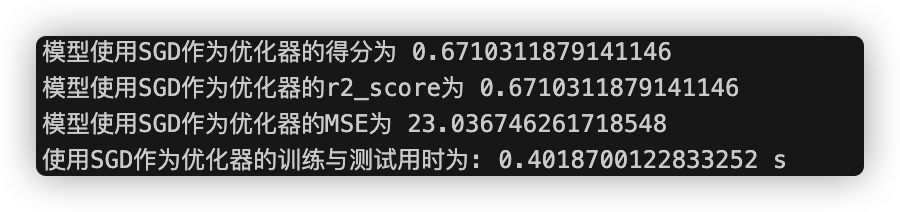
\includegraphics[width=0.7\textwidth,height=0.2\textwidth]{SGD.png}
	\caption{Results of linear regression by SGD}
\end{figure}
可以看出,数据的拟合效果十分良好,为了比较SGD方法与传统线性回归方法的差异,这里引入sklearn的LinearRegression方法,在同样的数据集上得到的结果如下:
\begin{figure}[H]
	\centering
	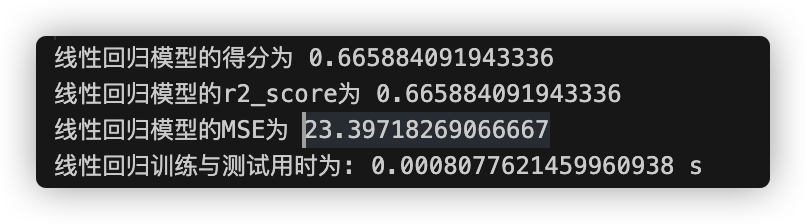
\includegraphics[width=0.7\textwidth,height=0.2\textwidth]{Linear.png}
	\caption{Results of linear regression by Linear}
\end{figure}
此时出现的现象十分奇怪,因为SGD方法反而速度更慢,查阅资料得知,LinearRegression采用的是SVD方法进行求解,当数据特征并不多,如本例,特征仅有$13$个时,其速度更快.为了更好地比较sklearn的几种线性回归方法,这里给出下表:
\begin{center}
\begin{tabular}{cccccc}
	\hline
	算法 & 训练实例数量$m$很大 & 特征数$n$很大 & 要求缩放 & Scikit-Learn \\
	\hline
	标准方程 & 快 & 慢 & 否 & None \\
	
	SVD & 快 & 慢 & 否 & LinearRegression \\
	
	SGD & 快 & 快 & 是 & SGDRegressor \\
	\hline
\end{tabular}
\end{center}
因此,可根据上表合适的选择回归器进行线性回归.
\end{sol}
\section{Ex5}
\textbf{对鸢尾花数据集利用$K$-均值聚类,计算轮廓系数.}
\begin{sol}
	首先,导入数据时选择导入数据的第$3,4$维,即叶子的宽度和长度,查阅资料知这是更加易于区分的性状.在导入数据后,调用sklearn.cluster的KMeans方法,选择超参数n\_clusters=3,可以得到聚类结果如下图所示,下图绘制了Voronoi图:
	\begin{figure}[H]
		\centering
		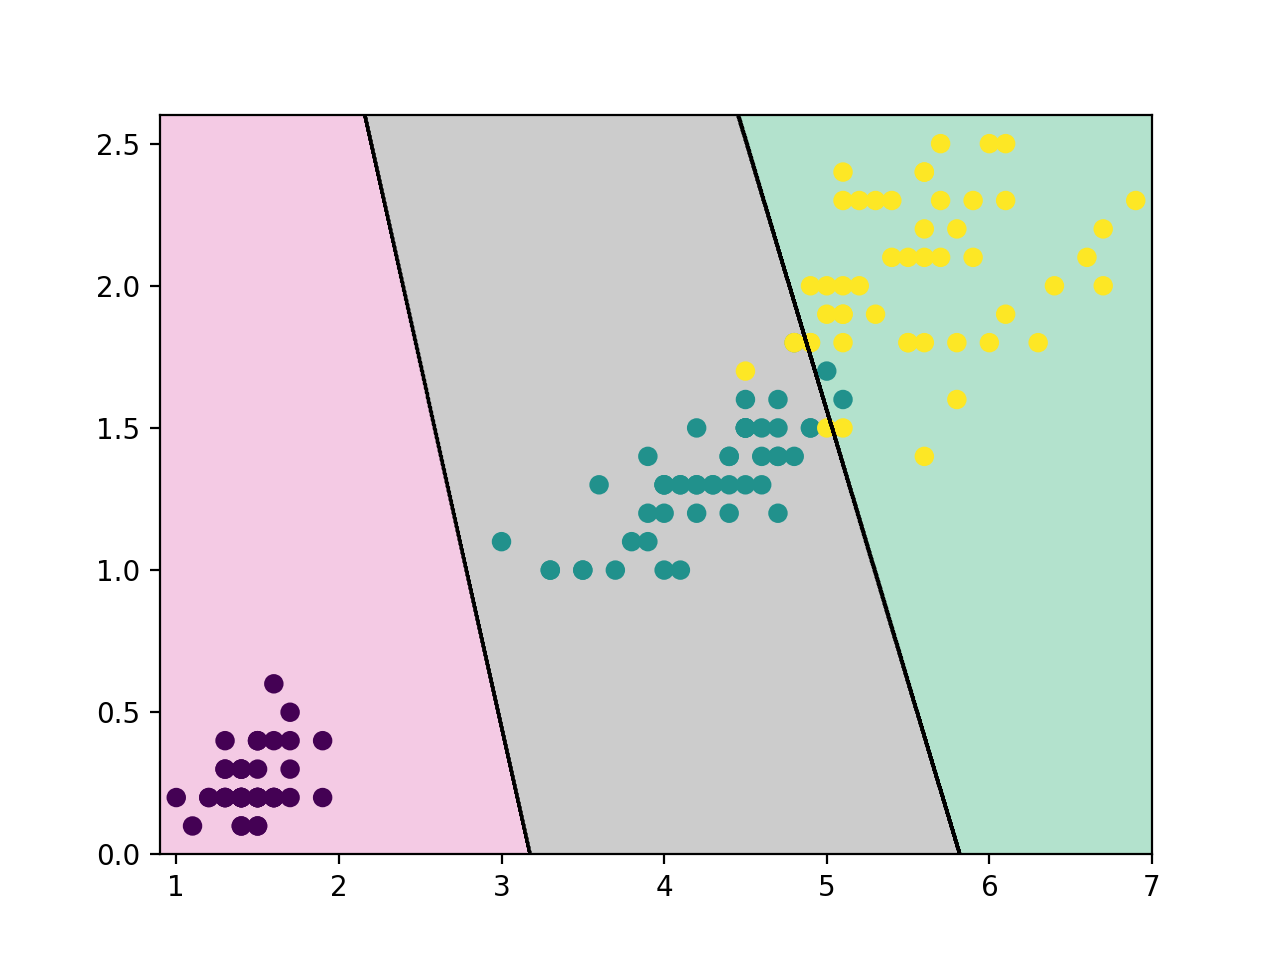
\includegraphics[width=0.7\textwidth,height=0.5\textwidth]{kmeans_v.png}
		\caption{Voronoi plot of K-means on iris when $k=3$}
	\end{figure}
	同时,可以计算得到轮廓系数为0.6604800083974887.
	而除了K-means聚类方法之外,还有Mini Batch K-means聚类方法,该算法的思想是在每次的迭代中使用小批量K-means稍微的移动中心点,而不是在每次迭代中使用完整的数据集,这使得迭代速度快了$3-4$倍,具体结果如下图所示:
	\begin{figure}[H]
		\centering
		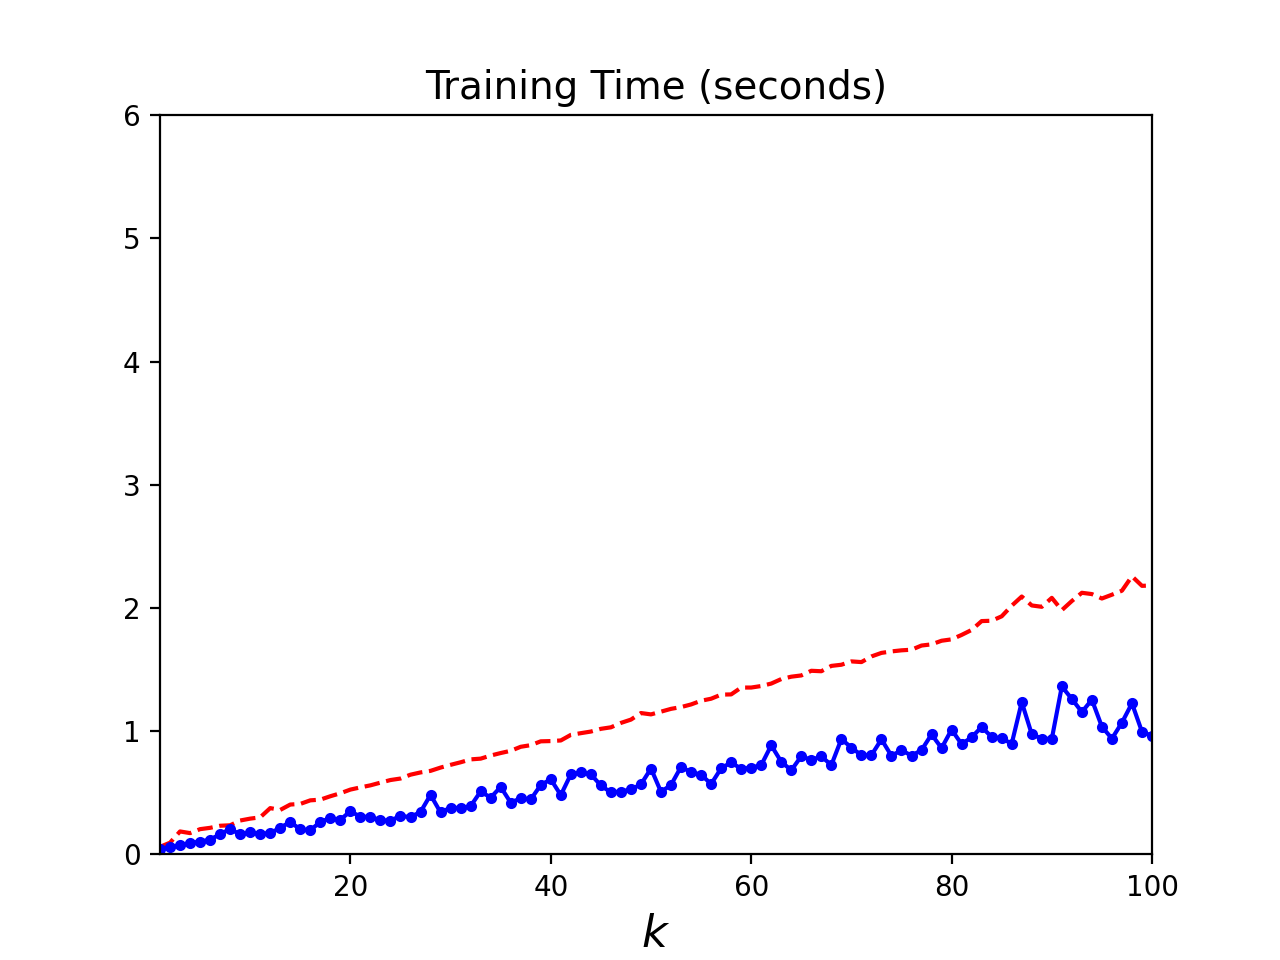
\includegraphics[width=0.7\textwidth,height=0.5\textwidth]{time.png}
		\caption{Training time of minibatch K-means vs K-menas}
	\end{figure}
\end{sol}
最后,考虑这样一个问题:如果不是根据经验,应当如何选取聚类的数量$k$呢?根据资料,答案往往是依据轮廓系数进行选择.因此,考虑绘制本问题轮廓系数随聚类数变化的曲线如图:
	\begin{figure}[H]
	\centering
	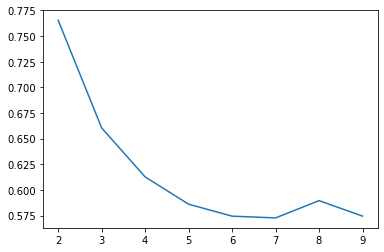
\includegraphics[width=0.6\textwidth,height=0.45\textwidth]{score.png}
	\caption{Silhouette score of different $k$}
\end{figure}
可以看出,对于本问题,事实上聚类为$2$类优于根据经验选择的$3$类,且聚类为$2$类的轮廓系数为0.7653904101258123,高于聚类为$3$类的轮廓系数.但这也反映出K-means算法的一个局限性,即必须多次运行算法才能避免次优解.
\newpage
\begin{thebibliography}{3}  
	\bibitem{ref1} 李航. 统计学习方法[M]. 清华大学出版社, 2012.
	%\bibitem{ref2} Kingma D , Ba J . Adam: A Method for Stochastic Optimization[J]. Computer Science, %2014.
	\bibitem{ref2} Goodfellow, Ian, et al. Deep Learning[M]. MIT Press, 2016. 	
	\bibitem{ref3} 周志华. 机器学习[M]. 清华大学出版社, 2013.
\end{thebibliography}
\end{document}
